\section{Cloud Services}
Ein Cloud-Dienst (englisch: Cloud Service) bezeichnet eine Dienstleistung, die von einem Cloud-Provider über das Internet bereitgestellt wird. Dabei stellt der Anbieter Ressourcen wie Compute, Speicher oder Software auf Abruf zur Verfügung, ohne dass der Nutzer eigene physische Infrastruktur betreiben muss.
\begin{figure}[H]
    \centering
    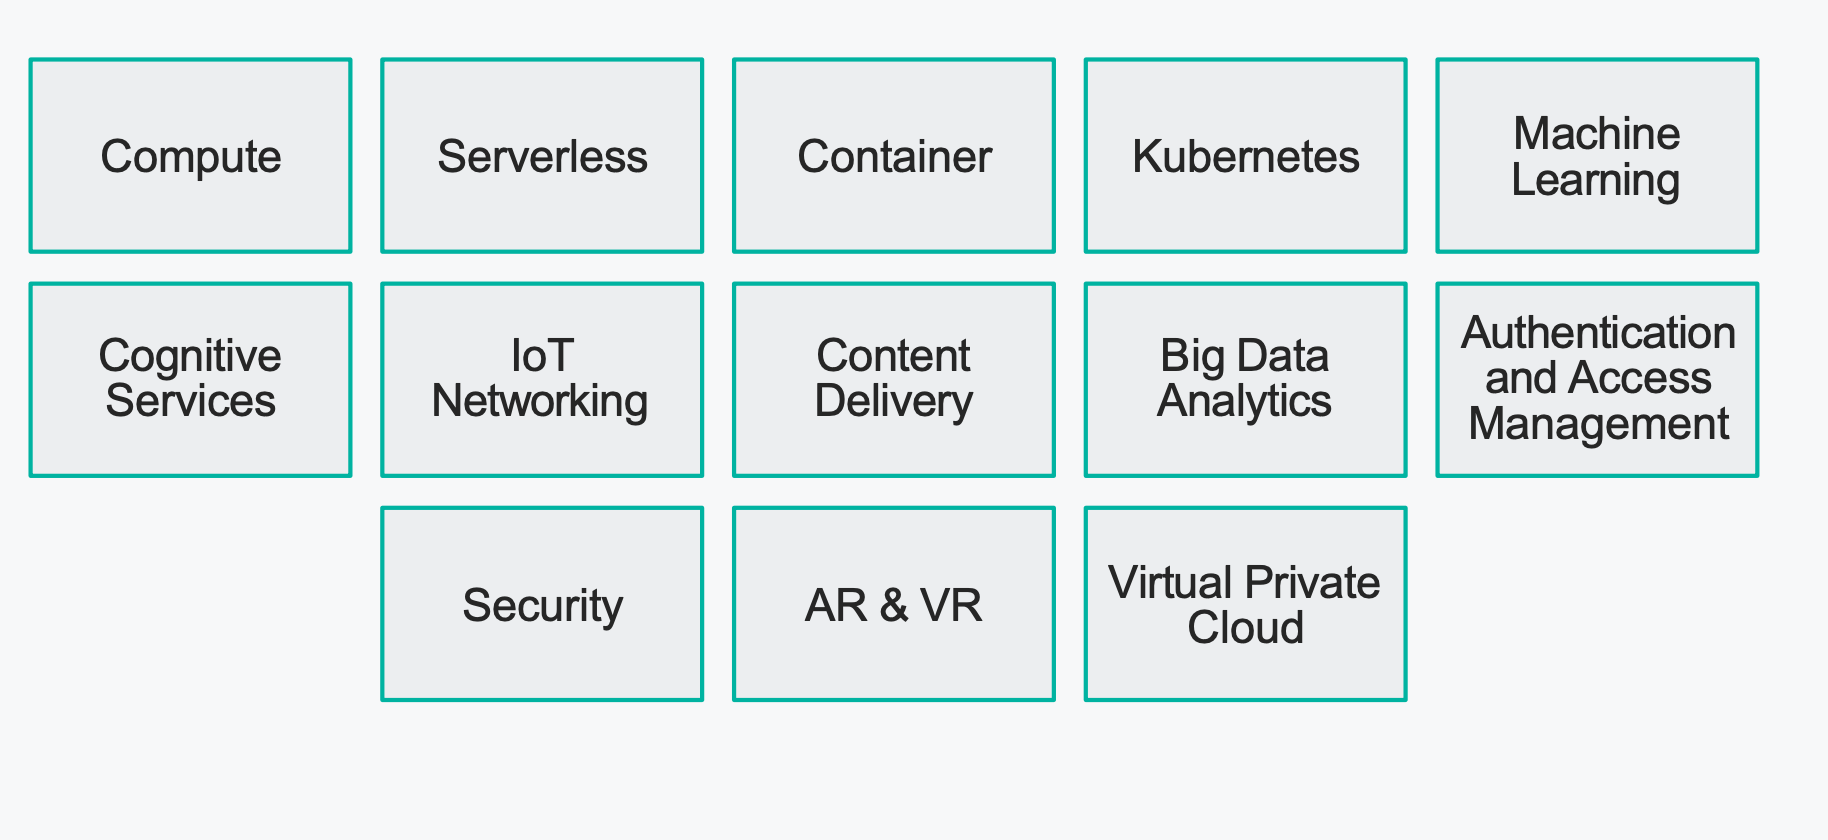
\includegraphics[width=\textwidth]{assets/images/TypischeCloudService}
    \caption{Grundlegende Services in Der Cloud}
\end{figure}
\subsection{Compute}
Compute bedeutet das bereitstellen von Rechenleistung. Also kann Compute hosten einer Webanwendung bedeutet oder des hosten eine KI modell wie Sonnet oder GPT 5 für ein Unternehmen.
\subsection{Serveless}
Serveless bedeutet das man Code ohne Pflege eines Server Hosten kann. Es ist oft teil von Ressourcen in Azure z.B. der Managed Service für Postgre Datenbanken. Ein sonder fall ist FaaS. Dies wird Später noch mal detailert erklärt.
  \begin{infobox}[Definiton FaaS – Function as a Service]
    FaaS baut auf Serveless auf und emrölicht Backend cod Serveless zu hosten, Durch Genreische sprachen wie z.B. Python. 
  \end{infobox}
\begin{table}[H]
  % \caption kommt VOR der Tabelle (FOM-Konvention)
  
  \label{tab:server-vs-serverless}

  % tabularx: streckt die Tabelle auf \textwidth
  % l = linksbündig, feste Breite (Aspekt-Spalte)
  % X = flexibel, füllt den Rest (die zwei Inhalts-Spalten)
  \begin{tabularx}{\textwidth}{|l|X|X|}
    \hline
    \textbf{Aspekt}
      & \textbf{Server Architecture}
      & \textbf{Serverless Architecture} \\
    \hline

    Infrastructure Management
      & Entwickler verwalten zugrunde liegende Server oder VMs.
      & Der Cloud-Anbieter verwaltet die Infrastruktur (Server). \\
    \hline

    Resource Allocation
      & Ressourcen, die basierend auf dem erwarteten Workload bereitgestellt werden.
      & Ressourcen, die dynamisch basierend auf dem Bedarf zugewiesen werden. \\
    \hline

    Scaling
      & Die Skalierung umfasst in der Regel manuelle oder automatisierte Prozesse.
      & Automatische Skalierung basierend auf Workload. \\
    \hline

    Cost Model
      & Die Kosten beinhalten Vorabinvestitionen und das laufende Management.
      & Pay-per-Use-Preismodell basierend auf Funktionsaufrufen. \\
    \hline

    State Management
      & Anwendungen behalten den Status auf der Serverseite bei.
      & Serverlose Funktionen sind von Natur aus zustandslos. \\
    \hline

  \end{tabularx}
  \caption{Vergleich Server Architecture und Serverless Architecture}

\end{table}
